\documentclass[12pt]{article}%
\usepackage[
  height=9in,      % height of the text block
  width=7in,       % width of the text block
  top=78pt,        % distance of the text block from the top of the page
  headheight=52pt, % height for the header block
  headsep=12pt,    % distance from the header block to the text block
  heightrounded,   % ensure an integer number of lines
  verbose,         % show the values of the parameters in the log file
]{geometry}%
\usepackage{array}%
\usepackage{multirow}%
\usepackage{fancyhdr}%
\usepackage{graphicx}%
\usepackage{tabularx}%
\setlength{\extrarowheight}{6pt}%
\usepackage{subcaption}%

%%%%%%%%%%%%%%%%%%%%%%%%%%%%%%%%%% HEADER AND FOOTER %%%%%%%%%%%%%%%%%%%%%%%%%%%%%%%%%%%
\pagestyle{fancy}
\fancyhf{\LARGE\textbf{Learn Basics} \\ \textbf{Chapter Report}}%
\rhead{Subject : \textbf{Math} \\ Class : \textbf{6} \\ Chapter : \textbf{5. Fractions}}%
\lhead{  
\includegraphics[width=1.5cm, height=1.5cm]{LearnBasics logo}  }{}%
\lfoot{\textbf{XYZ School}}%
\rfoot{XYZ1118 C6M05 CR##1}%
\cfoot{\thepage}

\renewcommand{\headrulewidth}{2pt}% Default \headrulewidth is 0.4pt
\renewcommand{\footrulewidth}{2pt}% Default \footrulewidth is 0pt 

\renewcommand{\arraystretch}{1}

\begin{document}
%%%%%%%%%%%%%%%%%%%%%%%%%%%%%%%%% 1ST STARTS FROM HERE %%%%%%%%%%%%%%%%%%%%%%%%%%%%%%%%%%%

\begin{center}
   \underline{\large\textbf{5. Fractions}} 
\end{center}
\vspace{0.5cm}{
\textbf{Chapter Start Date: }{20 Aug, 2022} \hspace{3cm} \textbf{Chapter End Date: }{20 Sept, 2022}}\\
\linebreak%
\begin{tabularx}{1\textwidth} { 
  | >{\centering\arraybackslash}X 
  | >{\centering\arraybackslash}X 
  | >{\centering\arraybackslash}X 
  | >{\centering\arraybackslash}X | }
 \hline
 \textbf{Total Students} & \textbf{Number of Quizzes} & \textbf{Class Performance} & \textbf{Class Attendance} \\[2ex]%
 \hline
30 & 5 & 66 & 96 \\[2ex]%
\hline
\end{tabularx}

\vspace{0.5cm}

\textbf{\begin{center}
\textbf{\underline{{Topic wise performance}}} 
\end{center}}\\
\vspace{0.2cm}
\begin{tabular}{
| >{}p{0.3\textwidth}
| >{\centering}p{0.16\textwidth}
| >{\centering}p{0.16\textwidth}
| >{\centering\arraybackslash}p{0.16\textwidth}| }
\hline
\multirow{1}{*}{\textbf{Topics}} & \multirow{1}{*}{\textbf{Performance}} & \multirow{1}{*}{\textbf{Attended}} & \multirow{1}{*}{\textbf{Yet to}}\\[1.5ex]%
\hline
 Basics of Fraction & & & \\[1ex]%
 \hline
 Types of Fraction & & & \\[1ex]%
 \hline
 Formation of Fraction & & & \\[1ex]%
 \hline
 Comparison of Fraction & & & \\[1ex]%
 \hline
 Operation of Fractions & & & \\[1ex]%
 \hline
 \end{tabular}
\vspace{0.35cm}%
\hline %
\vspace{0.35cm} %
\textbf{\begin{center}
\textbf{\underline{Performance Gap - Analysis}} \hspace{10cm} 
\end{center}} \\
\linebreak%
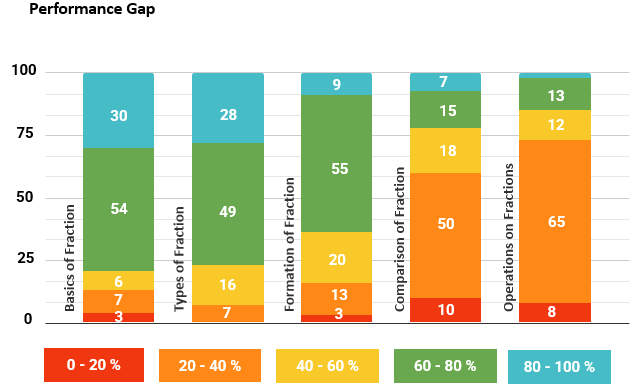
\includegraphics[width=16cm, height=8cm]{school report.png}

%%%%%%%%%%%%%%%%%%%%%%%%%%%%%%%%% 1ST PAGE ENDS %%%%%%%%%%%%%%%%%%%%%%%%%%%%%%%%%%%

%%%%%%%%%%%%%%%%%%%%%%%%%%%%%%%%% 2ND STARTS FROM HERE %%%%%%%%%%%%%%%%%%%%%%%%%%%%%%%%%%%
\begin{tabular}{
| >{\centering}p{0.05\textwidth}
| >{\centering}p{0.14\textwidth}
| >{\centering}p{0.1\textwidth}
| >{\centering}p{0.09\textwidth}
| >{\centering}p{0.14\textwidth}
| >{\centering}p{0.154\textwidth}
| >{\centering\arraybackslash}p{0.11\textwidth}| }
\hline
\multirow{1}{*}{S.No} & \multirow{1}{*}{Name} & \multirow{1}{*}{Basics of } \\ Fraction & \multirow{1}{*}{Types of}\\ Fraction & \multirow{1}{*}{Formation of} \\Fractions & \multirow{1}{*}{Comparision of} \\ Fraction & \multirow{1}{*}{Operation}\\[2.5ex]%
\hline
 & & & & & & \\[1.5ex]%
\hline
 & & & & & & \\[1.5ex]%
\hline
 & & & & & & \\[1.5ex]%
\hline
 & & & & & & \\[1.5ex]%
\hline
 & & & & & & \\[1.5ex]%
\hline
 & & & & & & \\[1.5ex]%
\hline
 & & & & & & \\[1.5ex]%
\hline
 & & & & & & \\[1.5ex]%
\hline
 & & & & & & \\[1.5ex]%
\hline
 & & & & & & \\[1.5ex]%
\hline
 & & & & & & \\[1.5ex]%
\hline
 & & & & & & \\[1.5ex]%
\hline
 & & & & & & \\[1.5ex]%
\hline
 & & & & & & \\[1.5ex]%
\hline
 & & & & & & \\[1.5ex]%
\hline
 & & & & & & \\[1.5ex]%
\hline
 & & & & & & \\[1.5ex]%
\hline
 & & & & & & \\[1.5ex]%
\hline
 & & & & & & \\[1.5ex]%
\hline
 & & & & & & \\[1.5ex]%
\hline
\end{tabular}
\vspace{5cm}
%%%%%%%%%%%%%%%%%%%%%%%%%%%%%%%%% 2ND PAGE ENDS %%%%%%%%%%%%%%%%%%%%%%%%%%%%%%%%%%%

%%%%%%%%%%%%%%%%%%%%%%%%%%%%%%%%%% 3RD PAGE STARTS FROM HERE %%%%%%%%%%%%%%%%%%%%%%%%%%%%%

\begin{center}
   \large \underline{{Homework Questions Report for} {Estimation of Numbers}}
\end{center}
\begin{center}
\underline{Concepts Tested in the Question:}
\end{center}
\begin{enumerate}
    \item Estimating to the nearest tens by rounding off
    \item Estimating to the nearest hundreds by rounding off
    \item Estimating to the nearest thousands by rounding off
\end{enumerate}

\vspace{1cm}\\

\begin{tabularx}{0.9\textwidth} { 
  | >{\centering\arraybackslash}X 
  | >{\centering\arraybackslash}X | }
 \hline
 Total Students & \textbf{30}\\
 \hline
 No.of Students attended the test  & \textbf{23}\\
\hline
 Absent & \textbf{7} \\
\hline
 Start Time & \textbf{7:00 PM - 15th May} \\
\hline
 End Time & \textbf{8:00 PM - 16th May} \\
\hline
 Total Questions & \textbf{5 - Basic Questions} \\
\hline
\end{tabularx}
\vspace{1.5cm}\\
%%%%%%%%%%% two tables side by side%%%%%%%%%%%%%%%%%%%%

    \begin{subtable}[t]{.6\textwidth}
    \caption{HELLO}
        \raggedright
            \begin{tabularx}{0.9\textwidth} { 
            | >{\centering\arraybackslash}X 
            | >{\centering\arraybackslash}X 
            | >{\centering\arraybackslash}X 
            | >{\centering\arraybackslash}X | }
            \hline
            \textbf{S.No} & \textbf{Name} & \textbf{Score} & \textbf{Time Taken} \\
            \hline
            1 & Arjun & 5 & 5:30min \\
            \hline
            1 & Bhanu & 5 & 5:00min \\
            \hline
            1 & Chandu & 3 & 4:30min \\
            \hline
            1 & Deepu & 4 & 2:30min \\
            \hline
            1 & Varun & 5 & 4:34min \\
            \hline
            \end{tabularx}
    \end{subtable}%
    \begin{subtable}[t]{.35\textwidth}
    \caption{HII}
        \raggedleft
        \begin{tabularx}{0.9\textwidth} { 
          | >{\centering\arraybackslash}X 
          | >{\centering\arraybackslash}X | }
         \hline
         \textbf{S.No} & \textbf{Name}\\
         \hline
         1 & Anind \\
         \hline
         2 & Bharath \\
         \hline
         3 & Code \\
         \hline
         4 & Drama \\
         \hline
         5 & Dheeraj \\
         \hline
         6 & Lohith \\
         \hline
         7 & Murali \\
         \hline
        \end{tabularx}
    \end{subtable}
%%%%%%%%%%%%%%%%%%%%%%%%%%%% 3RD PAGE ENDS %%%%%%%%%%%%%%%%%%%%%%%%%%%%%%%%%%%%%%%%%%%%

%%%%%%%%%%%%%%%%%%%%%%%%% 4TH PAGE STARTS FROM HERE%%%%%%%%%%%%%%%%%%%%%%%%%%%%%%%%%%%%%
\begin{tabular}{
| >{\centering}p{0.16\textwidth}
| >{\centering}p{0.32\textwidth}
| >{\centering}p{0.16\textwidth}
| >{\centering\arraybackslash}p{0.16\textwidth}| }
\hline
\multirow{1}{*}{S.No} & \multirow{1}{*}{Name} & \multirow{1}{*}{Score} & \multirow{1}{*}{Time Taken}\\[2ex]%
\hline
 & & & \\[1.5ex]%
 \hline
 & & & \\[1.5ex]%
 \hline
 & & & \\[1.5ex]%
 \hline
 & & & \\[1.5ex]%
 \hline
 & & & \\[1.5ex]%
 \hline
 & & & \\[1.5ex]%
 \hline
 & & & \\[1.5ex]%
 \hline
 & & & \\[1.5ex]%
 \hline
 & & & \\[1.5ex]%
 \hline
 & & & \\[1.5ex]%
 \hline
 & & & \\[1.5ex]%
 \hline
 & & & \\[1.5ex]%
 \hline
 & & & \\[1.5ex]%
 \hline
 & & & \\[1.5ex]%
 \hline
 & & & \\[1.5ex]%
 \hline
 & & & \\[1.5ex]%
 \hline
 & & & \\[1.5ex]%
 \hline
 & & & \\[1.5ex]%
 \hline
 & & & \\[1.5ex]%
 \hline
 & & & \\[1.5ex]%
 \hline
 & & & \\[1.5ex]%
 \hline
\end{tabular}
%%%%%%%%%%%%%%%%%%%%%%%%% 4TH PAGE ENDS %%%%%%%%%%%%%%%%%%%%%%%%%%%%%%%%%%%%%%%%%%%%%%%%
\end{document}